% =============================================================================
% ForensiQ — Wireframes / Protótipo de Navegação
% UC 21184 · Projeto de Engenharia Informática · UAb · 2025/26
% =============================================================================
\documentclass[a4paper,11pt]{article}

\usepackage[utf8]{inputenc}
\usepackage[T1]{fontenc}
\usepackage[portuguese]{babel}
\usepackage[top=2.2cm, bottom=2.2cm, left=2.2cm, right=2.2cm]{geometry}
\usepackage{graphicx}
\usepackage{booktabs}
\usepackage{longtable}
\usepackage{array}
\usepackage{parskip}
\usepackage{hyperref}
\usepackage{xcolor}
\usepackage{tcolorbox}
\usepackage{enumitem}
\usepackage{fancyhdr}

\definecolor{forensicblue}{HTML}{1E3A8A}
\definecolor{forensicgray}{HTML}{4B5563}

\hypersetup{
    colorlinks=true,
    linkcolor=forensicblue,
    urlcolor=forensicblue,
    pdfauthor={João Rodrigues},
    pdftitle={ForensiQ — Wireframes / Protótipo de Navegação}
}

\pagestyle{fancy}
\fancyhf{}
\fancyhead[L]{\small\textit{ForensiQ — Protótipo de Navegação}}
\fancyhead[R]{\small UC 21184 · 2025/26}
\fancyfoot[C]{\small\thepage}

\newcolumntype{L}[1]{>{\raggedright\arraybackslash}p{#1}}

\begin{document}

% =============================================================================
% Capa
% =============================================================================
\thispagestyle{empty}
\vspace*{2cm}
\begin{center}
    {\LARGE\bfseries Wireframes / Protótipo de Navegação}\\[0.6em]
    {\large ForensiQ --- Plataforma Modular de Gestão de Prova Digital\\
    para \textit{First Responders}}\\[2cm]

    \begin{tabular}{rl}
        \textbf{Estudante:}   & João M. M. Rodrigues · 2203474 \\
        \textbf{Orientador:}  & Prof. Pedro Duarte Pestana \\
        \textbf{Versão:}      & 1.0 · 3 de Maio de 2026 \\
        \textbf{Documento:}   & Cumprimento de \texttt{docs/design/wireframes.pdf} (guia §5) \\
    \end{tabular}
\end{center}

\vspace{2cm}

\begin{tcolorbox}[colback=forensicblue!5, colframe=forensicblue, title=\textbf{Nota metodológica}]
Este documento cumpre o item \texttt{docs/design/wireframes.pdf} listado como
\textbf{obrigatório para projectos com interface} no §5 do \textit{Guia de Projecto}
do orientador. Em alinhamento com o §7 (\textit{Opções metodológicas e desvios ao standard}),
o ForensiQ não seguiu a abordagem clássica de wireframes prévios em Figma/Balsamiq, mas sim
uma abordagem \textbf{iterativa \textit{code-first}} com revisões de design pós-implementação:

\begin{itemize}[nosep, leftmargin=*]
    \item \textbf{Sem 4-5} (7-20 abr) --- Implementação directa em HTML/CSS \textit{vanilla}
        com \textit{tokens} CSS centralizados, validada por \textit{stakeholder} (o próprio
        autor é o utilizador-tipo: perito digital forense da PSP).
    \item \textbf{Sem 6} (21-27 abr) --- \textit{Sweep} mobile-first, redesign \textit{Revolut-like}
        do \textit{wizard} de evidência e da \textit{landing page}.
    \item \textbf{Sem 6} (18 abr) --- Auditoria de design estruturada
        (\href{auditoria-de-design.html}{\texttt{auditoria-de-design.html}}, 34 achados),
        que substitui formalmente o protótipo prévio.
    \item \textbf{Sem 7} (28 abr-3 mai) --- Redesign do \textit{dashboard} e da \textit{custody timeline}
        com base nos achados; mode tabela densa para \textit{desktop} (PR \#1+\#2).
\end{itemize}

A justificação para esta abordagem: o autor é simultaneamente desenvolvedor e utilizador-tipo
(perito da PSP), eliminando a necessidade de validação prévia com utilizadores externos via
wireframes de baixa fidelidade. O documento abaixo apresenta as vistas-chave \textbf{tal como
implementadas} a 3 mai 2026 e o mapa de navegação consolidado.
\end{tcolorbox}

\newpage

% =============================================================================
% Mapa de navegação
% =============================================================================
\section{Mapa de navegação}

O sistema tem três camadas de navegação:

\begin{enumerate}[leftmargin=*]
    \item \textbf{Pública} --- apenas \texttt{/login/}.
    \item \textbf{Autenticada (qualquer perfil)} --- \texttt{/dashboard/}, listagens
        (\texttt{/occurrences/}, \texttt{/evidences/}, \texttt{/custodies/}),
        páginas de detalhe, \texttt{/stats/}, \texttt{/reports/}, \texttt{/settings/}.
    \item \textbf{Autenticada (apenas AGENT)} --- formulários de criação
        (\texttt{/occurrences/new/}, \texttt{/evidences/new/}) e transições de custódia.
\end{enumerate}

\subsection*{Fluxo principal --- caso de uso \textit{first responder}}

\begin{tcolorbox}[colback=gray!5, colframe=forensicgray]
\texttt{/login/} \\
\hspace*{1em}$\downarrow$ autenticação JWT (\textit{cookies} HttpOnly + CSRF) \\
\texttt{/dashboard/} \\
\hspace*{1em}$\downarrow$ acção rápida ``Nova Ocorrência'' \\
\texttt{/occurrences/new/} \quad (\textit{wizard} 6-\textit{step}, GPS automático) \\
\hspace*{1em}$\downarrow$ submissão $\rightarrow$ HTTP 201 + \textit{redirect} \\
\texttt{/occurrences/<id>/} \quad (\textit{hub} do caso) \\
\hspace*{1em}$\downarrow$ acção ``Adicionar item de prova'' \\
\texttt{/evidences/new/?occurrence=<id>} \quad (\textit{wizard} 18 tipos, foto, GPS, IMEI/VIN \textit{lookup}) \\
\hspace*{1em}$\downarrow$ submissão $\rightarrow$ \textit{hash} SHA-256 calculado \\
\texttt{/evidences/<id>/} \quad (detalhe com \textit{hash} + custódia actual) \\
\hspace*{1em}$\downarrow$ ``Avançar custódia'' \\
\texttt{/evidences/<id>/custody/} \quad (\textit{timeline} cronológica, modal de transição)
\end{tcolorbox}

\subsection*{Fluxo do perito --- após chegada ao laboratório}

\begin{tcolorbox}[colback=gray!5, colframe=forensicgray]
\texttt{/dashboard/} \\
\hspace*{1em}$\downarrow$ \textit{filter} ``Em trânsito'' \\
\texttt{/custodies/} \\
\hspace*{1em}$\downarrow$ marcar como recebida \\
\texttt{/evidences/<id>/custody/} $\rightarrow$ transição \textit{RECEBIDA\_LABORATORIO} $\rightarrow$ \textit{EM\_PERICIA} \\
\hspace*{1em}$\downarrow$ \textit{export} relatório \\
\texttt{/api/evidences/<id>/pdf/} \quad (PDF forense ReportLab + declaração ISO/IEC 27037)
\end{tcolorbox}

\newpage

% =============================================================================
% Vistas-chave
% =============================================================================
\section{Vistas-chave (estado a 3 mai 2026)}

\subsection{Dashboard --- redesign (versão actual, desktop)}

\textit{Layout} \textit{wide} com \textit{stats} de cadeia de custódia em barra horizontal,
acções rápidas e últimas ocorrências. Resultado da auditoria 18 abr + \textit{sweep} 28 abr-3 mai.

\begin{center}
    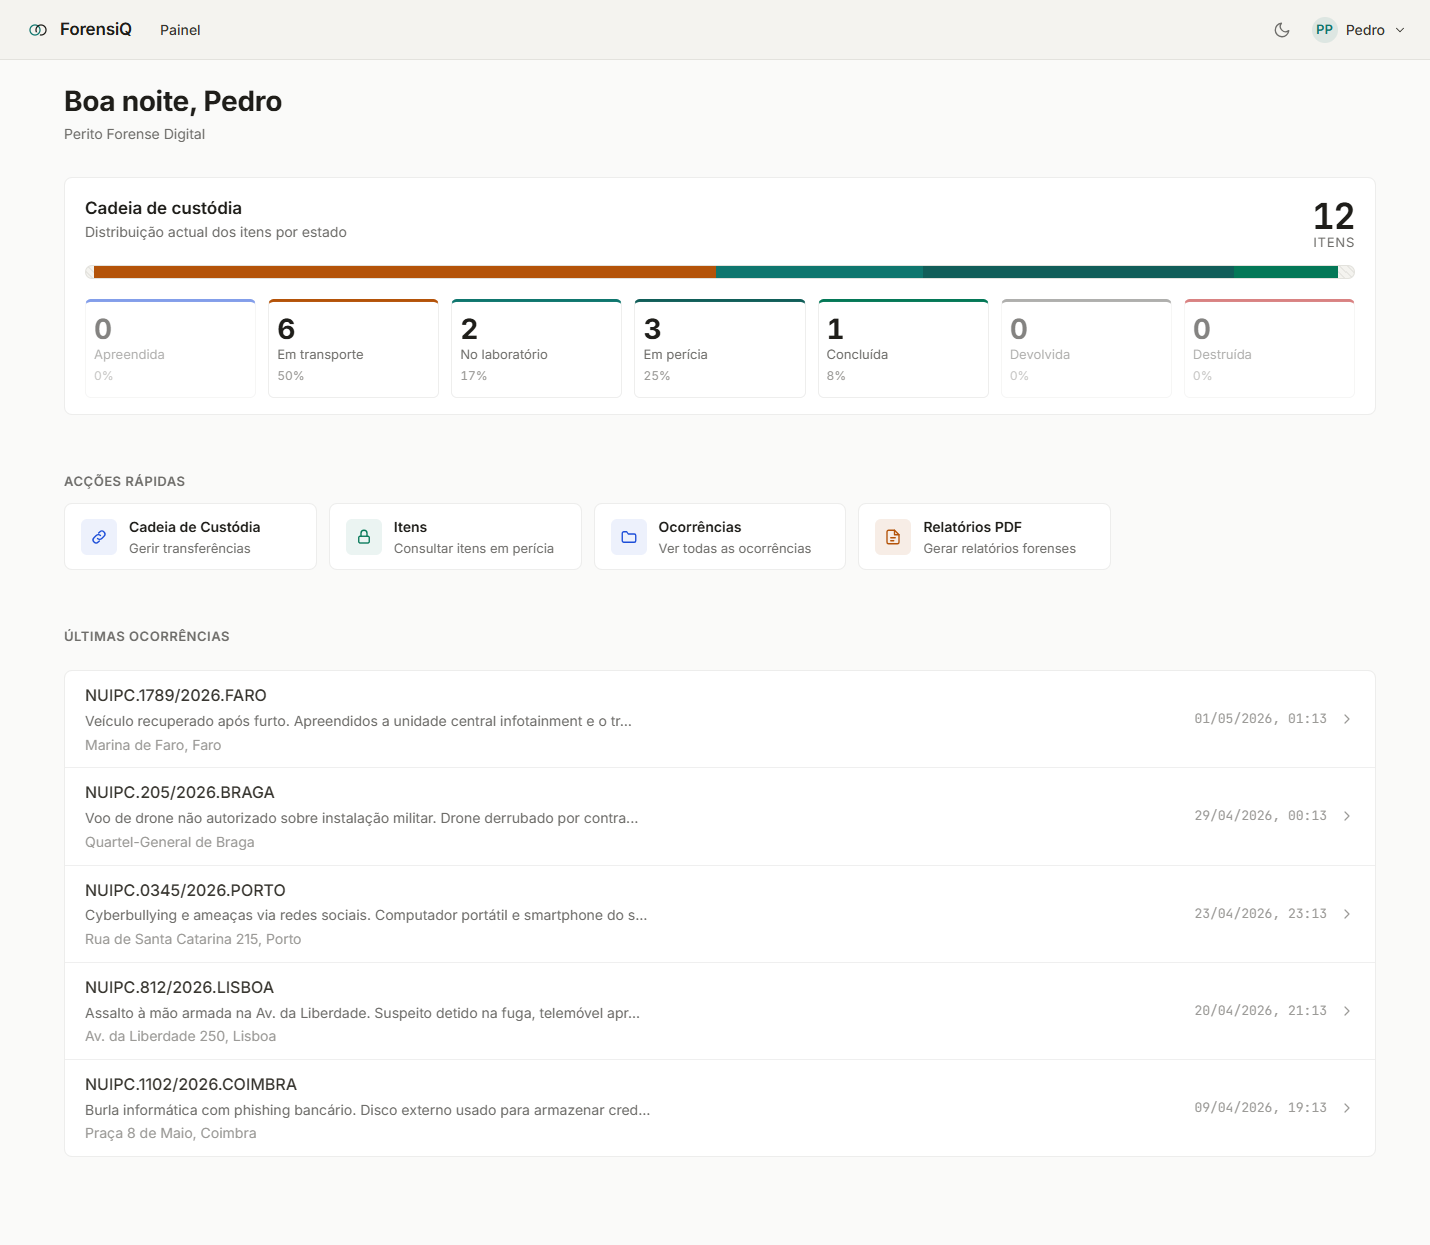
\includegraphics[width=0.95\textwidth]{screens/dashboard-redesign.png}
\end{center}

\subsection{Timeline de custódia --- redesign (desktop)}

\textit{Timeline} cronológica com \textit{state progress} e \textit{hashes} SHA-256
encadeados. Modal de transição (apenas AGENT, próximo estado válido).

\begin{center}
    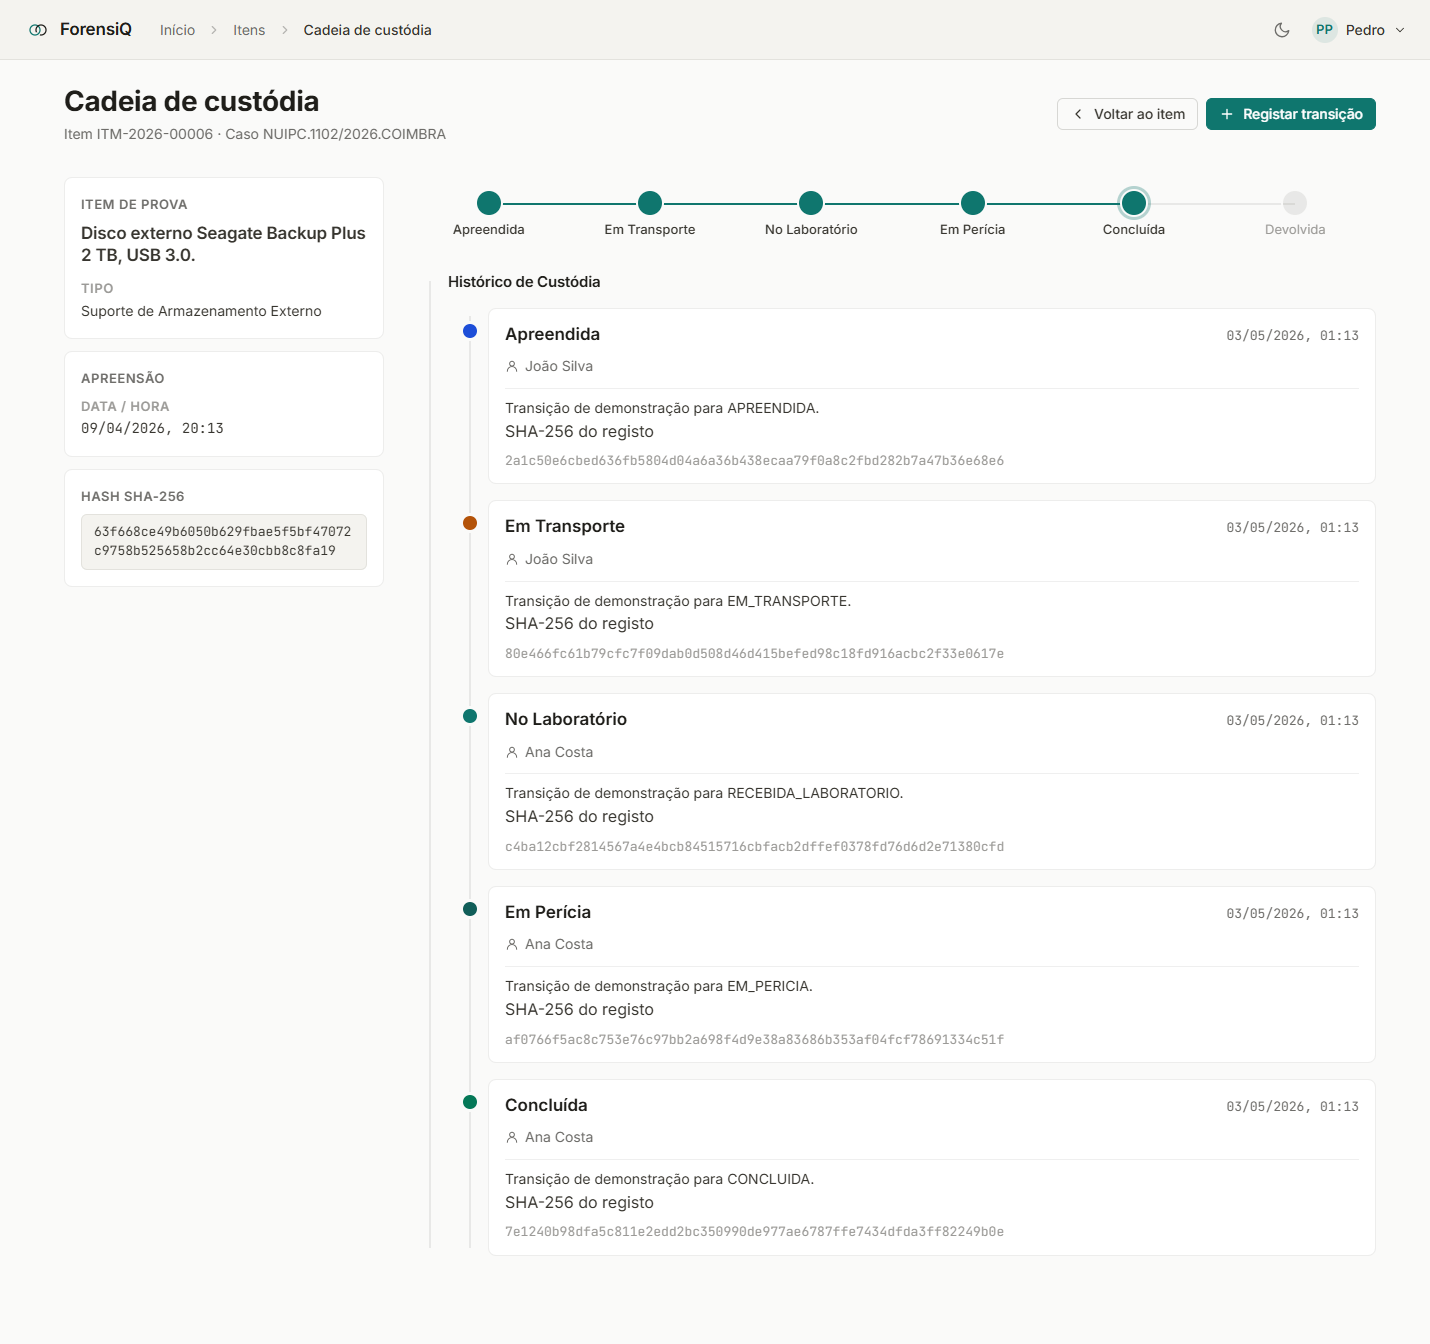
\includegraphics[width=0.95\textwidth]{screens/custody-timeline-redesign.png}
\end{center}

\clearpage

\subsection{Vistas mobile (perito no terreno)}

À esquerda, \textit{dashboard} reordenado (acções rápidas em destaque).
Ao centro, listagem de cadeia de custódia adaptada a mobile (filtros compactos).
À direita, \textit{navbar} colapsada (\textit{brand} ``ForensiQ'' visível $\geq$ 340px;
\textit{touch targets} $\geq$ 48px, WCAG 2.1 AA).

\vspace{0.6em}

\noindent\begin{minipage}[t]{0.32\textwidth}
\centering
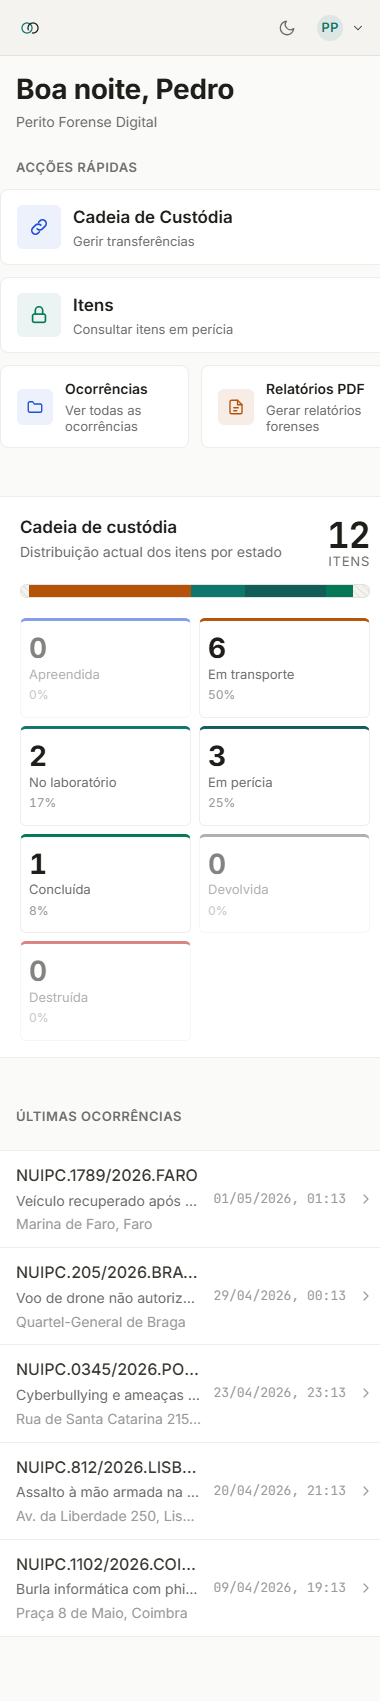
\includegraphics[width=\linewidth, height=0.62\textheight, keepaspectratio]{screens/dashboard-mobile-reordered.png}\\[0.3em]
{\small\textit{Dashboard mobile}}
\end{minipage}\hfill
\begin{minipage}[t]{0.32\textwidth}
\centering
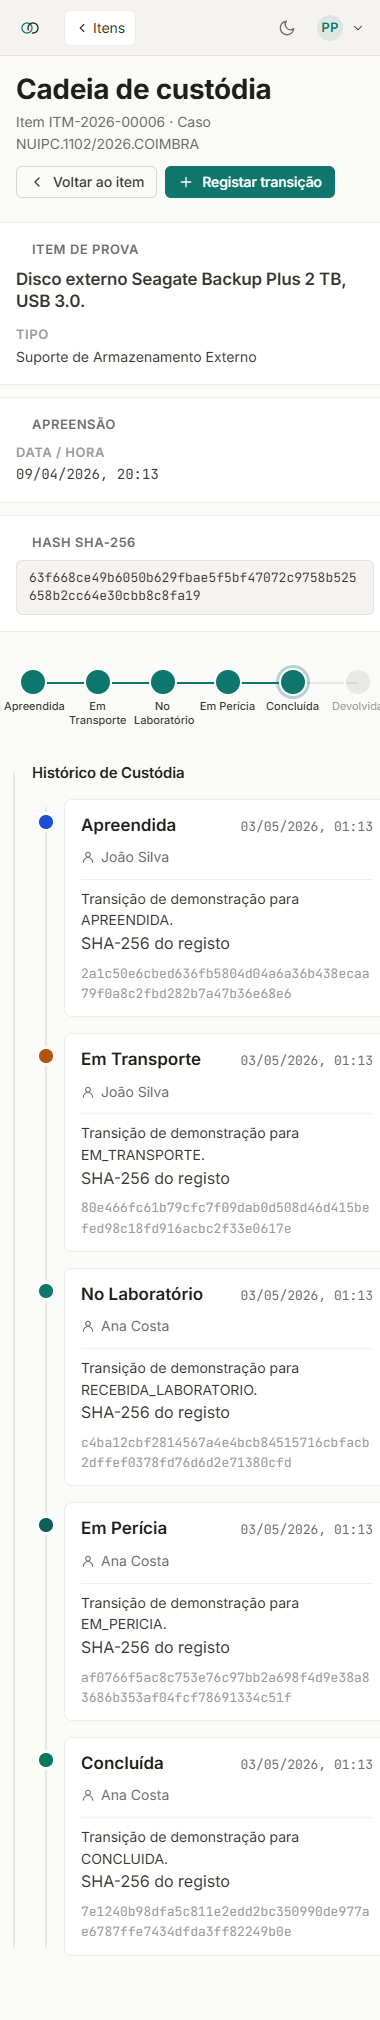
\includegraphics[width=\linewidth, height=0.62\textheight, keepaspectratio]{screens/custody-mobile.png}\\[0.3em]
{\small\textit{Cadeia de custódia mobile}}
\end{minipage}\hfill
\begin{minipage}[t]{0.32\textwidth}
\centering
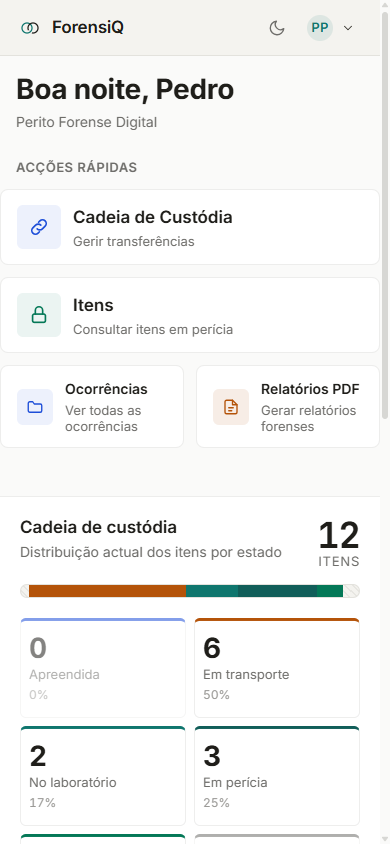
\includegraphics[width=\linewidth, height=0.62\textheight, keepaspectratio]{screens/navbar-mobile.png}\\[0.3em]
{\small\textit{Navbar colapsada}}
\end{minipage}

% =============================================================================
% Princípios
% =============================================================================
\section{Princípios de design aplicados}

\begin{itemize}[leftmargin=*]
    \item \textbf{Mobile-first com escala desktop} --- decisões de layout começam pelo
        viewport mais constrangido (perito no terreno com luvas) e expandem para desktop.
    \item \textbf{Touch targets $\geq$ 48px} --- conformidade WCAG 2.1 AA.
    \item \textbf{Tokens CSS centralizados} --- toda a paleta, espaçamento e tipografia
        em \texttt{main.css} (\textit{dark mode} automático ao entardecer via NOAA \textit{sunset calc}).
    \item \textbf{Tipografia funcional} --- Inter para UI, JetBrains Mono para
        \textit{hashes}, IDs e \textit{timestamps} (legibilidade em campo forense).
    \item \textbf{Tokens semânticos por estado} --- cada estado da cadeia de custódia
        (\texttt{APREENDIDA}, \texttt{EM\_TRANSPORTE}, etc.) tem cor própria
        (\texttt{--state-apreendida}, ...).
    \item \textbf{Acessibilidade} --- \texttt{aria-busy}, \texttt{aria-pressed},
        \textit{live regions} para anúncios, \textit{roving tabindex} em \textit{radiogroups}.
\end{itemize}

% =============================================================================
% Próximos passos
% =============================================================================
\section{Próximos passos (Sem 9-13)}

\begin{itemize}[leftmargin=*]
    \item Validação com 2-3 peritos da PSP fora do círculo do autor (Sem 11-12).
    \item Testes de usabilidade em terreno simulado (Sem 13).
    \item Polimento final com base no \textit{feedback} (Sem 13).
\end{itemize}

\vspace{1cm}
\hrule
\vspace{0.5em}
\begin{center}
\small\textit{Ver também:} \href{auditoria-de-design.html}{\texttt{auditoria-de-design.html}}
(34 achados estruturados, 18 abr 2026) \\
\textit{e ADR-0004} (\href{../architecture/adr/ADR-0004-frontend-architecture.md}{\texttt{ADR-0004-frontend-architecture.md}})
\end{center}

\end{document}
